\subsection{Filter Design}

The typical Human can only hear frequencies in the range of 20Hz through 20kHz, and this range only decreases as humans age  \cite{human:rg}.  Using the website \url{http://onlinetonegenerator.com/hearingtest.html}, we will test the hearing range of each member listening to our final presentation.  This demonstration will provide a tangible example why appropriate filtering of an audio signal will have little to no impact on the quality of sound that a person hears after the filtering.  

When our project group performed the hearing test, the highest audible frequency was 15kHz.  Since our project group was not able to hear the frequencies above the 15kHz threshold, any low pass filter that removed the high frequencies above 15kHz would have no impact on what we hear.  Removing the unecessary frequencies from an audio signal transmission provides a few nice benefits such as the following: 

\begin{enumerate}
\item It reduces the necessary power for transmission of the audio signal
\item It reduces the necessary bandwidth for transmission
\end{enumerate}

Given the human threshold for hearing, an obvious opportunity is to apply low-pass filtering in order to transmit audio signals with smaller bandwidths.  The ideal low pass filter would completely eliminate all frequencies above a certain cutoff point (in our hearing test example, the cutoff would be at 15kHz) while passing all frequencies below the cutoff point \cite{lowpass:wiki}.     

In order to filter out higher frequencies in an audio signal transmission, we will build a low pass filter.  Specifically, we will describe how a low pass filter is created using a finite number of non-zero filter coefficients which is called a \textit{Finite Impulse Response} filter or FIR.  Given the impulse response, we can find the coefficients of the filter, and vice versa \cite{notes:class}.  For example, Figure \ref{fig:lowpass} shows a graphical depiction of a low pass filter that begins to cut out the frequencies above 1 rad/s.  Frequencies below the cutoff frequency are considered to be in the ``Passband," or allowable frequency band.  Frequencies above the cutoff frequency filtered out and are considered in the ``Stopband."  

\begin{figure}[h!]
	\centering
	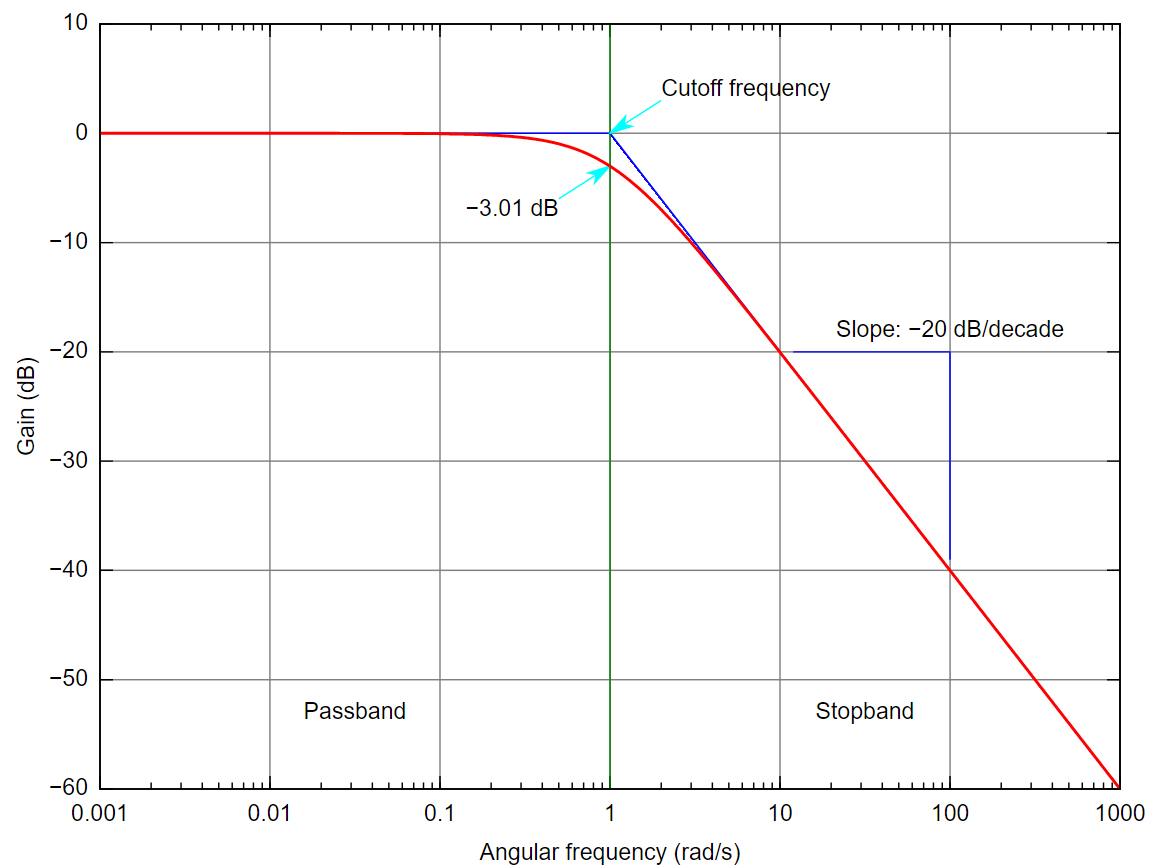
\includegraphics[scale = .5]{low_pass.png} %this is useful too \includegraphics[width = \linewidth]
	\caption{Example of Low Pass Filter: \url{https://upload.wikimedia.org/wikipedia/commons/6/60/Butterworth_response.svg}}
	\label{fig:lowpass}
\end{figure}    
 
